% ============================================================
% Template LaTeX para Trabalhos Acadêmicos
% Instituto Federal do Paraná – Campus Pinhais
% APÊNDICE K – Modelo de Trabalho Acadêmico para Projeto de Curso I
%
% Baseado na estrutura do template UTFPR-PG (abntex2)
% Adaptado para o modelo do IFPR Campus Pinhais
% ============================================================



\documentclass{ifpr-pinhais}

% \usepackage{cmap}
\usepackage{amsmath}
\usepackage{graphicx}
\usepackage{latexsym}
\usepackage{amssymb}
\usepackage{placeins}

\graphicspath{{imagens/}}

% ---- Metadados do trabalho ----
\curso{Bacharelado em Ciência da Computação}
\departamento{Coordenação do Curso de Bacharelado em Ciência da Computação}
\autor{Rafael Correia Alves \\ João Pedro dos Santos Henrique Plinta}
\titulo{Monitoramento de Funções Virtualizadas de Redes: Um Estudo Comparativo entre Ferramentas de Extração de Comportamento}
\tipotrabalho{Trabalho de Conclusão de Curso}
\local{Pinhais}
\data{2026}

\orientador{Prof. Guilherme Werneck de Oliveira}
% \coorientador{Prof. Nome do Coorientador}  % descomente se houver

\preambulo{%
  \imprimirtipotrabalho\ apresentado como requisito parcial para
  obtenção do título de Bacharel em \imprimircurso, do
  \ifpr\ -- \campus.
}

% ---- Configurações do PDF ----
\makeatletter
\hypersetup{
  pdftitle={\@title},
  pdfauthor={\@author},
  pdfsubject={\imprimirpreambulo},
  pdfcreator={LaTeX com abntex2 e ifpr-pinhais},
  hidelinks,
}
\makeatother

% ---- Espaçamento entre parágrafos ----
\setlength{\parskip}{0.1cm}

\makeindex

% ============================================================
\begin{document}
\frenchspacing

% ================================================================
% ELEMENTOS PRÉ-TEXTUAIS
% ================================================================
\pretextual

% --- Capa ---
\imprimircapa

% --- Folha de Rosto ---
\imprimirfolhaderosto

% --- Folha de Aprovação ---
% (preencha com os dados reais antes de imprimir)
\imprimirfolhadeaprovacao

% --- Dedicatória (opcional) ---
% \begin{dedicatoria}
%   \vspace*{\fill}
%   \centering
%   \noindent
%   \textit{Dedico este trabalho...}
%   \vspace*{\fill}
% \end{dedicatoria}

% --- Agradecimentos (opcional) ---
% \begin{agradecimentos}
%   Agradeço...
% \end{agradecimentos}

% --- Epígrafe (opcional) ---
% \begin{epigrafe}
%   \vspace*{\fill}
%   \begin{flushright}
%     \textit{``Frase de efeito.''\\(Autor, Ano)}
%   \end{flushright}
% \end{epigrafe}

% --- Resumo em português --- (pendente: escrever após Desenvolvimento)
% \begin{resumo}
%   Conter de 150 e 500 palavras, em parágrafo único com espaçamento simples,
%   tamanho 12, sem recuo na primeira linha. Deve-se ressaltar sucintamente o
%   conteúdo de um texto: os objetivos, os métodos empregados, os resultados
%   preliminares e as conclusões. Recomenda-se para documento técnico e científico
%   o resumo informativo.
%
%   \vspace{\onelineskip}
%   \noindent
%   \textbf{Palavras-chave}: palavra 1; palavra 2; palavra 3; palavra 4; palavra 5.
% \end{resumo}

% --- Abstract (resumo em inglês) --- (pendente)
% \begin{resumo}[Abstract]
%   \begin{otherlanguage*}{english}
%     Mandatory element, written preferably in English. It must contain the same
%     information as the Portuguese abstract, including keywords.
%
%     \vspace{\onelineskip}
%     \noindent
%     \textbf{Keywords}: word 1; word 2; word 3; word 4; word 5.
%   \end{otherlanguage*}
% \end{resumo}

% --- Lista de Figuras (a partir de 5 figuras) ---
\pdfbookmark[0]{\listfigurename}{lof}
\listoffigures*
\cleardoublepage

% --- Lista de Gráficos (a partir de 5 gráficos) --- (pendente)
% \pdfbookmark[0]{Lista de Gráficos}{log}
% \listof{grafico}{Lista de Gráficos}
% \cleardoublepage

% --- Lista de Tabelas (a partir de 5 tabelas) ---
\pdfbookmark[0]{\listtablename}{lot}
\listoftables*
\cleardoublepage

% --- Lista de Quadros (opcional) ---
% \pdfbookmark[0]{Lista de Quadros}{loq}
% \listof{quadro}{Lista de Quadros}
% \cleardoublepage

% --- Lista de Abreviaturas e Siglas ---
\begin{siglas}
  \item[BCC]   BPF Compiler Collection
  \item[BPF]   Berkeley Packet Filter
  \item[CPU]   Central Processing Unit
  \item[eBPF]  Extended Berkeley Packet Filter
  \item[IFPR]  Instituto Federal do Paraná
  \item[NFV]   Network Functions Virtualization
  \item[RTT]   Round-Trip Time
  \item[TCP]   Transmission Control Protocol
  \item[UDP]   User Datagram Protocol
  \item[VNF]   Virtualized Network Function
  \item[WAF]   Web Application Firewall
  \item[MANO]  Management and Orchestration
\end{siglas}

% --- Lista de Símbolos (opcional) ---
% \begin{simbolos}
%   \item[$\Gamma$] Letra grega Gama
% \end{simbolos}

% --- Sumário ---
\pdfbookmark[0]{\contentsname}{toc}
\tableofcontents*
\cleardoublepage

% ================================================================
% ELEMENTOS TEXTUAIS
% ================================================================
\textual
\pagestyle{simple}

% ----------------------------------------------------------------
\input{capítulos/0.Introdução}
\input{capítulos/1.RevisãoDaLiteratura}

\chapter{Metodologia}
\label{chap:metodologia}

Esta pesquisa é classificada como \textbf{aplicada}, pois tem como finalidade gerar conhecimento direcionado à solução de um problema prático específico: a escolha de ferramentas de monitoramento adequadas para ambientes de virtualização de funções de rede \cite{gil2021}. Quanto à abordagem, é \textbf{quantitativa}, uma vez que os dados coletados são expressos numericamente e submetidos a tratamento estatístico \cite{marconi2017}. Em relação aos seus objetivos, caracteriza-se como \textbf{comparativa}, pois visa estabelecer diferenças e semelhanças de desempenho entre as três abordagens estudadas. Por fim, quanto ao procedimento técnico, trata-se de uma \textbf{pesquisa experimental}, na qual as variáveis são controladas e os efeitos de diferentes tratamentos são mensurados sob condições padronizadas \cite{gil2021}.

%\section{Classificação da Pesquisa}



\section{Contexto Experimental}

As VNFs voltadas para a segurança, como os WAF e os IDS, são os elementos mais beneficiados pelo uso do eBPF \cite{technologies12080122}. Em um WAF tradicional, a análise de pacotes exige que todo o tráfego passe por validações de assinaturas no espaço do usuário, sobrecarregando a CPU sob ataques DDoS, por exemplo.

Projetos como o \textit{CODAX} (\textit{Container-aware DDoS Attack detection using eXtended Berkeley Packet Filter}) mostram que o eBPF pode realizar a detecção precoce de ataques direcionados à exaustão de CPU de forma altamente eficiente \cite{codax2025remya}. O CODAX monitora o consumo de tempo de CPU de processos a partir do momento em que a chamada de sistema \texttt{accept()} é executada, registrando timestamps em um mapa global. Esse mecanismo permite identificar conexões maliciosas antes mesmo do término da conexão, \texttt{close()}, reduzindo a latência de detecção em 94,2\% em comparação com abordagens tradicionais e operando de forma estável sob carga.

Além disso, arquiteturas híbridas de WAF dividem as responsabilidades de inspeção: o eBPF atua no kernel filtrando conexões conhecidamente maliciosas através de listas negras armazenadas em mapas rápidos, enquanto delega requisições suspeitas complexas para o motor WAF em espaço de usuário \cite{hybridvnf2017}. Caso o WAF no espaço de usuário identifique um padrão malicioso, ele atualiza dinamicamente o mapa eBPF, permitindo que todos os pacotes subsequentes daquela origem sejam descartados instantaneamente no \textit{kernel}. Esses casos de uso evidenciam que o WAF, por concentrar carga computacional em inspeções de conteúdo intensivas em CPU, constitui uma VNF representativa para avaliar o impacto do monitoramento: qualquer sobrecarga adicional introduzida pelo coletor concorre diretamente com os recursos destinados à inspeção de tráfego, tornando visíveis mesmo pequenas diferenças entre as abordagens avaliadas \cite{10.1145/3397022}.

Conforme discutido na Seção~\ref{subsec:requisitos_monitoramento}, há uma particularidade dos ambientes de NFV diretamente relacionada ao escopo deste trabalho: o observador não atua como um agente externo à infraestrutura, mas executa co-localizado à VNF, compartilhando os mesmos núcleos de CPU e a mesma memória do \textit{host}. Em consequência, a sobrecarga imposta pela própria ferramenta de monitoramento --- e não apenas o impacto indireto que ela provoca sobre a VNF --- constitui objeto central de comparação: um coletor que consuma recursos em excesso compete diretamente com a função de rede que deveria apenas observar, degradando justamente o serviço que se pretende proteger \cite{10.1145/3397022}. Por essa razão, as métricas de tempo de resposta, CPU e memória do próprio observador, e não somente as do WAF, são tratadas como variáveis dependentes centrais neste estudo.

Os experimentos foram conduzidos em uma máquina física com processador AMD Ryzen 5 5500 (6 núcleos e 12 \textit{threads}, frequência máxima de 4,27 GHz, \textit{cache} L3 de 16 MB), 16 GB de memória RAM, sistema operacional Ubuntu 26.04 LTS (\textit{Resolute Raccoon}) e kernel Linux versão 7.0.0-15-\textit{generic}. Os principais componentes de software utilizados estão descritos na Tabela~\ref{tab:versoes_software}.

\begin{table}[htbp]
\centering
\caption{Versões dos componentes de software utilizados nos experimentos.}
\label{tab:versoes_software}
\begin{tabularx}{\textwidth}{lX}
\hline
\textbf{Componente} & \textbf{Versão / Origem} \\
\hline
Kernel Linux (host e contêineres) & 7.0.0-15-\textit{generic} (Ubuntu 26.04 LTS; compartilhado por todos os contêineres Docker) \\
Python, observadores e WAF & 3.12.3 (\texttt{ubuntu:24.04}) \\
Python, cliente           & 3.9 (\texttt{python:3.9-slim}) \\
libbpf                     & 1.3.0 (\texttt{libbpf1} 1:1.3.0-2build2, repositório Ubuntu 24.04) \\
Compilador eBPF            & clang 18.1.3 (\texttt{1ubuntu1}, repositório Ubuntu 24.04) \\
psutil                     & 7.2.2 (via pip, instalada no contêiner) \\
prometheus\_client         & 0.25.0 (via pip, instalada no contêiner) \\
matplotlib                 & 3.10.9 (via pip, instalada no host para geração de gráficos) \\
numpy                      & 2.4.6 (via pip, instalada no host para geração de gráficos) \\
Docker Engine              & 29.5.3 (repositório oficial Docker CE) \\
\hline
\end{tabularx}
\end{table}

O isolamento entre os experimentos é garantido por três pilhas Docker Compose independentes, cada qual em seus próprios contêineres: o cliente, o WAF e o observador. O contêiner do coletor eBPF requer modo privilegiado (\texttt{privileged: true}), acesso ao PID do host (\texttt{pid: host}) e montagem do sistema de arquivos BPF (\texttt{/sys/fs/bpf}), necessários para carregar e executar programas no kernel. Os coletores Sysstat e Prometheus operam em modo não privilegiado, mas também com \texttt{pid: host}, para que a biblioteca \texttt{psutil} possa localizar e monitorar o processo WAF em execução na máquina alvo.

\section{Topologia e Arquitetura do Experimento}

A topologia adotada é composta por três elementos principais --- cliente, WAF e observador ---, além do \texttt{probe.py}, responsável por aferir o tempo de resposta do observador, todos ilustrados na Figura~\ref{fig:arquitetura_c4}. O fluxo de comunicação entre os três elementos principais segue a ordem:

\begin{enumerate}
    \item \textbf{Cliente:} envia cargas pré-geradas ao WAF via conexões TCP persistentes na porta 8080, utilizando 200 rotinas assíncronas (funções que podem ser suspensas e retomadas cooperativamente pelo laço de eventos, permitindo concorrência sem múltiplas \textit{threads} de sistema operacional). O protocolo de enquadramento utiliza um prefixo de 4 bytes em ordem de bytes big-endian indicando o tamanho da carga, com múltiplas mensagens por conexão;
    % CORREÇÃO overflow: BLOCKED e waf_metrics.json quebrados com \linebreak[0]
    \item \textbf{WAF:} inspeciona cada carga em busca de padrões maliciosos, injeção de SQL (SQLi), scripts entre sítios (XSS), travessia de caminho (\textit{Path Traversal}), execução remota de código (RCE) e byte nulo (\textit{Null Byte}), usando \texttt{asyncio} com \texttt{Thread\-Pool\-Executor}; responde \texttt{ALLOWED:OK} ou \texttt{BLOCKED:\-<mo\-ti\-vo>} e persiste métricas de inspeção em \texttt{waf\_met\-rics.\-json} a cada 100 requisições;
    \item \textbf{Observador:} mantém um \textit{socket} UDP servidor na porta 9999 e, ao receber uma requisição (pacote UDP enviado periodicamente pelo \texttt{probe.py} para medir o tempo de resposta do coletor), lê as métricas de rede e do processo WAF, respondendo com um objeto JSON contendo os valores coletados.
\end{enumerate}

\begin{figure}[htbp]
    \centering
    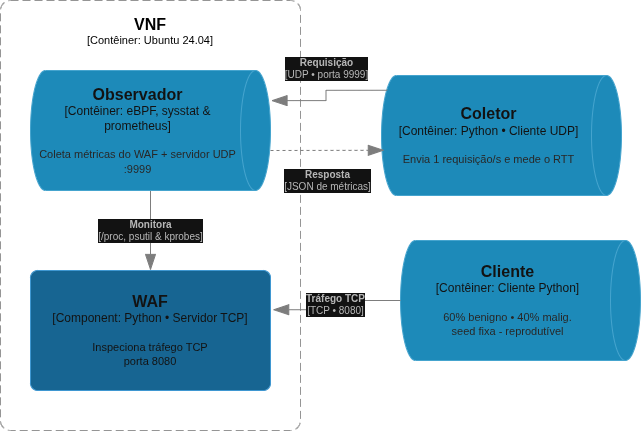
\includegraphics[width=0.85\textwidth]{imagens/C4model.drawio.png}
    \caption{Diagrama de contêineres (C4, Nível 2) da topologia experimental.}
    \label{fig:arquitetura_c4}
\end{figure}

O processo de medição é realizado pelo \texttt{probe.py}, que envia uma requisição UDP a cada 1 segundo para o observador ativo. O tempo de ida e volta é medido com resolução de nanossegundos via \texttt{time.time\_ns()}, sendo esta a métrica primária de sobrecarga do monitoramento. Antes de iniciar a coleta, o \texttt{probe.py} aguarda até 60 segundos pela disponibilidade do observador, garantindo que nenhuma amostra seja registrada antes da inicialização completa do coletor.

\section{Implementação dos Coletores}

\subsection{Coletor eBPF}

O coletor eBPF utiliza a biblioteca \textit{libbpf} com a abordagem CO-RE, que elimina a dependência do arcabouço BCC/LLVM em tempo de execução e permite que o programa BPF compilado seja portável entre versões de kernel compatíveis \cite{gregg_bpf_2019}. O programa em C (\texttt{ebpf\_kern.c}) é compilado para \textit{bytecode} eBPF durante a construção da imagem Docker e carregado no kernel na inicialização do observador.

Dois programas são anexados por meio de \textit{kprobes}: (a) \texttt{kprobe/tcp\_sendmsg}: intercepta cada chamada de envio TCP, acumulando os bytes transmitidos (TX) para conexões cuja porta de origem é 8080; e (b) \texttt{kprobe/tcp\_cleanup\_rbuf}: intercepta a liberação do \textit{buffer} de recepção TCP, acumulando os bytes recebidos (RX) para a mesma porta. Os contadores são armazenados em mapas eBPF do tipo \texttt{HASH}, chaveados pelo identificador da conexão. O processo em espaço do usuário lê esses contadores de forma assíncrona a cada solicitação recebida, sem cópias de pacotes e sem pressão adicional sobre a pilha de rede.

\subsection{Coletor Sysstat}

O coletor Sysstat opera de forma reativa: a cada requisição UDP recebida, lê o arquivo \texttt{/proc/net/dev} e extrai os contadores acumulados de bytes RX e TX da interface de loopback (\texttt{lo}), calculando o delta em relação ao valor inicial para estimar o tráfego acumulado desde o início do experimento \cite{godard2024sysstat}. O consumo de CPU e de memória do processo WAF é obtido pela biblioteca \texttt{psutil}, que consulta os arquivos \texttt{/proc/<pid>/stat} e \texttt{/proc/<pid>/status}.

\subsection{Coletor Prometheus}

% CORREÇÃO overflow: /proc/net/dev quebrado com \linebreak[0]
O coletor Prometheus adota a mesma lógica de coleta do Sysstat (leitura de \texttt{/proc/\linebreak[0]net/dev} e \texttt{psutil}), com o acréscimo de um servidor HTTP na porta 8000, implementado com a biblioteca \texttt{prometheus\_client} do Python \cite{turnbull_prometheus_2018}. Esse servidor expõe as métricas coletadas no formato padrão Prometheus via \texttt{/metrics}, habilitando a integração com um servidor de coleta externo. Neste experimento, nenhum servidor Prometheus externo realiza a coleta das métricas: o \textit{endpoint} permanece disponível, mas não é consultado durante os testes, o que restringe o escopo à sobrecarga do processo exporter em si, excluindo o custo do ciclo completo de \textit{scraping} presente em implantações reais. A sobrecarga adicional em relação ao Sysstat decorre exclusivamente da presença do servidor HTTP em execução, que consome ciclos de CPU para manter o \textit{socket} aberto e serializar as métricas a cada atualização interna.

O código-fonte dos três coletores, da geração de carga e da análise estatística está disponível publicamente no GitHub\footnote{https://github.com/joaopedroplinta/vnf-monitoring-benchmark}.

\section{Protocolo de Testes e Geração de Carga}

Neste experimento, o volume de mensagens N constitui a variável independente, assumindo quatro níveis: 100.000, 500.000, 1.000.000 e 2.000.000. A variável dependente primária é o tempo de resposta do observador (RTT UDP); CPU e memória do WAF e do coletor são variáveis dependentes secundárias, utilizadas para caracterizar a sobrecarga de cada abordagem.

As cargas são geradas previamente pelo script \texttt{gen\_payloads.py}, que produz arquivos binários com N mensagens nos quatro volumes citados. Cada arquivo contém 60\% de cargas benignas (textos aleatórios com caracteres ASCII imprimíveis) e 40\% de cargas maliciosas, intercaladas aleatoriamente com semente fixa \texttt{42} (\texttt{--seed 42}), garantindo que a sequência de mensagens seja idêntica entre ferramentas e volumes, condição necessária para a validade comparativa do experimento. O cliente lê as cargas sob demanda via fila assíncrona, mantendo o consumo de memória constante independentemente do volume N. A duração de cada execução é calculada de acordo com a Equação \ref{eq:duration}:

\begin{equation}
\text{DURATION} = \lfloor N / 15000 \rfloor + 20 \text{ segundos}
\label{eq:duration}
\end{equation}

O divisor 15.000 corresponde à taxa de vazão sustentada empiricamente pelas 200 corrotinas assíncronas no ambiente de testes, expressa em mensagens por segundo; os 20 segundos adicionais constituem uma margem de segurança para a inicialização e o encerramento dos contêineres. Esse valor garante que o cliente complete o envio de todas as cargas e que o observador capture amostras suficientes para a análise. Para cada combinação de coletor e volume N, foram realizadas \textbf{30 repetições} independentes, totalizando 360 execuções (3 coletores $\times$ 4 volumes $\times$ 30 repetições). Cada repetição executa o ciclo completo: inicialização dos contêineres, aquecimento do observador, coleta de dados e encerramento controlado via \texttt{docker compose down}.

Em cinco das 360 execuções, verificou-se \texttt{inspect\_count = 0} e \texttt{inspect\_avg\_ms = 0}, causados por uma condição de execução na leitura do arquivo \texttt{waf\_metrics.json}: o \texttt{probe.py} encerrou a coleta antes de o WAF gravar o arquivo pela primeira vez naquela execução. O critério adotado foi o seguinte: como a condição de execução afeta exclusivamente a leitura do arquivo \texttt{waf\_metrics.json} e não o mecanismo de requisição UDP, as medições de tempo de resposta UDP dessas execuções são válidas e estão incluídas nas agregações da métrica primária, preservando o tamanho amostral de 30 repetições para essa métrica; as métricas de inspeção (\texttt{inspect\_count}, \texttt{inspect\_avg\_ms}, \texttt{inspect\_min\_ms}, \texttt{inspect\_max\_ms}) dessas cinco execuções, cujos valores são zero por definição e não refletem o comportamento real do WAF, são desconsideradas nas análises de inspeção do WAF para não distorcer as médias.

\section{Métricas Coletadas e Análise Estatística}

O \texttt{probe.py} registra, a cada requisição, as seguintes métricas \cite{rfc8172}:

\begin{itemize}
    \item \textbf{Tempo de resposta do observador} (\texttt{observador\_latency\_avg\_ms}): tempo de ida e volta da requisição UDP em milissegundos, constituindo a métrica primária de sobrecarga do monitoramento;
    \item \textbf{CPU do WAF} (\texttt{cpu\_avg\_pct}): consumo médio de CPU do processo WAF durante o experimento;
    \item \textbf{Memória do WAF} (\texttt{mem\_avg\_mb}): consumo médio de memória RSS do processo WAF;
    \item \textbf{CPU do observador} (\texttt{collector\_cpu\_avg\_pct}): consumo médio de CPU do próprio observador;
    \item \textbf{Memória do observador} (\texttt{collector\_mem\_avg\_mb}): consumo médio de memória RSS do observador;
    \item \textbf{Bytes RX/TX} (\texttt{bytes\_rx}, \texttt{bytes\_tx}): volume acumulado de bytes recebidos e transmitidos. Não são diretamente comparáveis entre as ferramentas, pois o coletor eBPF contabiliza apenas o tráfego do WAF (filtrando \texttt{sport = 8080} no \textit{kernel}), enquanto o Sysstat e o Prometheus medem todo o tráfego da interface de \textit{loopback};
    % CORREÇÃO overflow: \raggedright local no item com os três \texttt longos
    \item {\raggedright\textbf{Métricas de inspeção do WAF}: contagem total de inspeções (\texttt{inspect\_count}), tempo médio, mínimo e máximo por inspeção (\texttt{inspect\_avg\_ms}, \texttt{inspect\_min\_ms}, \texttt{inspect\_max\_ms}).\par}
\end{itemize}

Destas, as cinco primeiras (tempo de resposta, CPU e memória do WAF e do observador) constituem as \textbf{métricas de comparação} entre as abordagens, conforme a discussão da Seção~\ref{subsec:requisitos_monitoramento}. As duas últimas (bytes RX/TX e métricas de inspeção) são \textbf{métricas de validação e caracterização}: confirmam que as três ferramentas processaram a mesma carga e caracterizam o custo de inspeção do WAF, mas não compõem a comparação entre coletores --- seja por independerem do coletor empregado (tempo de inspeção), seja por não serem mutuamente comparáveis (bytes RX/TX).

Os resultados das 30 repetições são agregados pelo script \texttt{compare.py}, que calcula a \textbf{média aritmética} e o \textbf{intervalo de confiança de 95\%} (IC95\%) para cada métrica, utilizando a distribuição t de Student \cite{marconi2017}. O IC95\% é calculado pela Equação \ref{eq:ic95}.

\begin{equation}
\text{IC}_{95\%} = t_{(n-1;\;0{,}025)} \cdot \frac{s}{\sqrt{n}}
\label{eq:ic95}
\end{equation}

\noindent onde $n = 30$ é o número de repetições, $s$ é o desvio padrão amostral entre as repetições e $t_{(29;\;0{,}025)} = 2{,}045$ é o quantil da distribuição t de Student bicaudal com $n - 1 = 29$ graus de liberdade e nível de significância $\alpha = 0{,}05$. Os resultados são apresentados no formato $\bar{x} \pm \text{IC}_{95\%}$, onde $\bar{x}$ é a média das 30 repetições. Os resultados finais são exportados nos formatos CSV e JSON para análise comparativa entre as três ferramentas.

Reconhecem-se as seguintes limitações dos experimentos: (i) o tráfego que flui pela interface de loopback (\texttt{lo}), o que elimina o overhead de drivers de NIC físico presentes em ambientes de produção; isso implica que os valores absolutos de latência UDP e de bytes RX/TX são inferiores ao que se observaria em uma rede física, onde interrupções de hardware e transferências DMA adicionam carga à CPU e aumentam a variância das medições; (ii) todos os contêineres compartilham o mesmo kernel e núcleos de CPU, de modo que contenção de recursos entre cliente, WAF e observador é possível; (iii) o WAF é uma implementação simplificada em Python, cujo perfil de CPU difere de soluções de produção como o ModSecurity. Contudo, por ser idêntico em todos os experimentos, garante que as diferenças observadas entre os coletores reflitam exclusivamente o custo de cada abordagem de monitoramento, e não características da VNF em si. Esses fatores limitam a generalização direta dos resultados absolutos, sem prejuízo à validade comparativa entre as três abordagens avaliadas sob as mesmas condições.

\chapter{Resultados}
\label{chap:resultados}

Este capítulo apresenta os resultados das 360 execuções realizadas, organizados em torno da métrica primária de sobrecarga, o tempo de resposta do observador (RTT UDP), e das métricas secundárias de consumo de recursos (CPU e memória do WAF e do próprio coletor). Todos os valores são apresentados no formato $\bar{x} \pm \text{IC}_{95\%}$, conforme a metodologia descrita no Capítulo~\ref{chap:metodologia}, e foram agregados pelo \texttt{compare.py} a partir das 30 repetições de cada combinação de coletor e volume $N$.

\section{Tempo de Resposta do Observador}

O tempo de resposta do observador, que mede o tempo de ida e volta da requisição UDP até a entrega das métricas coletadas, constitui a variável dependente primária deste estudo. A Tabela~\ref{tab:rtt} consolida os valores médios para os quatro volumes de mensagens avaliados, e a Figura~\ref{fig:rtt_barras} os representa graficamente.

\begin{table}[htbp]
\centering
\caption{Tempo de resposta médio do observador (RTT UDP, em ms) por volume de mensagens.}
\label{tab:rtt}
\begin{tabular}{lccc}
\hline
\textbf{Volume ($N$)} & \textbf{eBPF} & \textbf{Sysstat} & \textbf{Prometheus} \\
\hline
100.000   & $0{,}5407 \pm 0{,}0121$ & $0{,}6012 \pm 0{,}0048$ & $0{,}6205 \pm 0{,}0046$ \\
500.000   & $0{,}5038 \pm 0{,}0055$ & $0{,}5721 \pm 0{,}0034$ & $0{,}5844 \pm 0{,}0042$ \\
1.000.000 & $0{,}4885 \pm 0{,}0039$ & $0{,}5725 \pm 0{,}0053$ & $0{,}5682 \pm 0{,}0026$ \\
2.000.000 & $0{,}5283 \pm 0{,}0070$ & $0{,}5746 \pm 0{,}0037$ & $0{,}5932 \pm 0{,}0042$ \\
\hline
\end{tabular}
\end{table}

\begin{figure}[htbp]
    \centering
    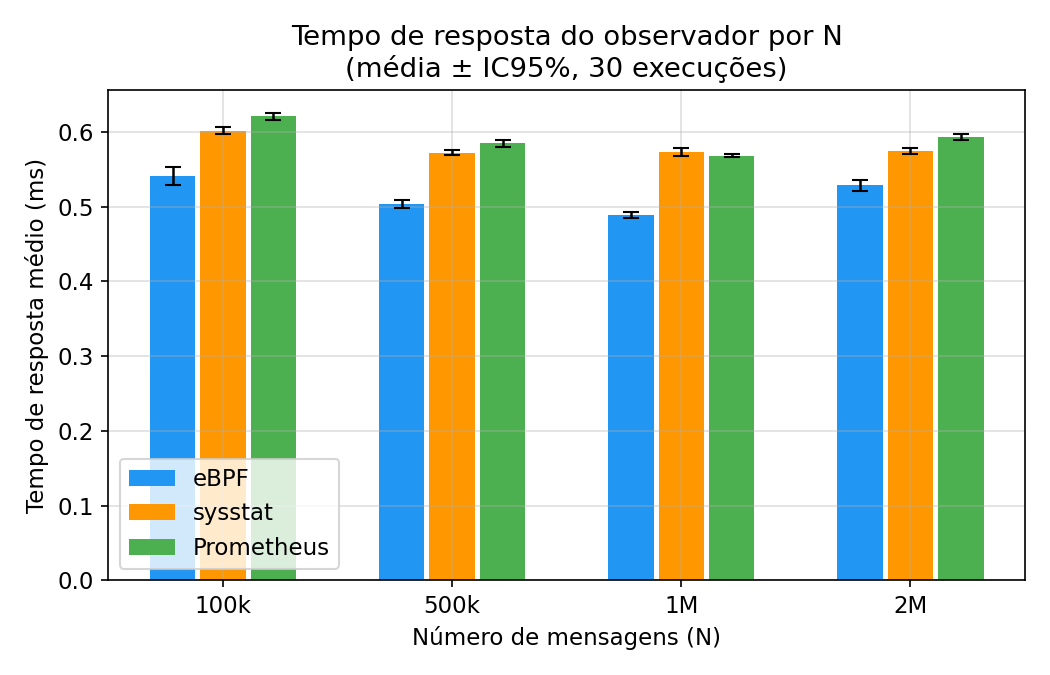
\includegraphics[width=0.85\textwidth]{imagens/tempo_resposta_por_n.png}
    \caption{Tempo de resposta médio do observador por volume de mensagens.}
    \label{fig:rtt_barras}
\end{figure}

O eBPF apresentou o menor tempo de resposta em todos os volumes avaliados. As reduções em relação ao Sysstat variaram de 8,1\% ($N = 2$ milhões) a 14,7\% ($N = 1$ milhão), e em relação ao Prometheus de 10,9\% ($N = 2$ milhões) a 14,0\% ($N = 1$ milhão). Em nenhum dos quatro volumes os intervalos de confiança de 95\% do eBPF se sobrepõem aos das demais ferramentas, indicando que a vantagem observada é estatisticamente significativa ao nível $\alpha = 0{,}05$. Esse comportamento é coerente com a natureza da abordagem: o coletor eBPF lê contadores previamente acumulados em mapas no \textit{kernel}, sem efetuar varreduras de arquivos do \texttt{/proc} nem serializar as métricas a cada requisição, ao passo que os coletores Sysstat e Prometheus realizam, a cada requisição, a leitura e o \textit{parsing} de \texttt{/proc/net/dev} e a consulta a \texttt{psutil} no espaço de usuário.

Entre Sysstat e Prometheus, as diferenças são pequenas e nem sempre consistentes: o Prometheus foi ligeiramente mais lento em três dos quatro volumes, o que é compatível com o custo adicional de manter o servidor HTTP ativo. Em $N = 1$ milhão, contudo, os dois coletores praticamente se igualaram ($0{,}5725$ \textit{vs.} $0{,}5682$ ms), com intervalos de confiança sobrepostos, de modo que não se pode afirmar diferença significativa entre eles nesse ponto.

Observa-se também que o tempo de resposta não cresce de forma monotônica com o volume de mensagens. Para as três ferramentas, os menores valores ocorrem em volumes intermediários ($N = 500$ mil e $N = 1$ milhão), enquanto $N = 100$ mil apresenta os maiores tempos médios. Esse efeito decorre da curta duração das execuções de menor volume, em que a fase de inicialização e estabilização do \textit{cache} representa fração maior do experimento; com volumes maiores, o sistema opera por mais tempo em regime estacionário, reduzindo a média.

A Figura~\ref{fig:rtt_boxplot} detalha a distribuição das execuções por meio de diagramas de caixa. Confirma-se a separação clara entre o eBPF e os demais coletores: em $N = 500$ mil e $N = 1$ milhão, a caixa do eBPF situa-se inteiramente abaixo das caixas de Sysstat e Prometheus, sem sobreposição. Nota-se, por outro lado, que o eBPF apresenta maior dispersão entre execuções, caixas mais largas e \textit{outliers} ocasionais, como o valor máximo de $1{,}0622$ ms em $N = 2$ milhões, enquanto os coletores em espaço de usuário exibem distribuições mais concentradas. Ainda assim, mesmo seus piores casos típicos permanecem competitivos com a mediana das demais ferramentas.

\begin{figure}[htbp]
    \centering
    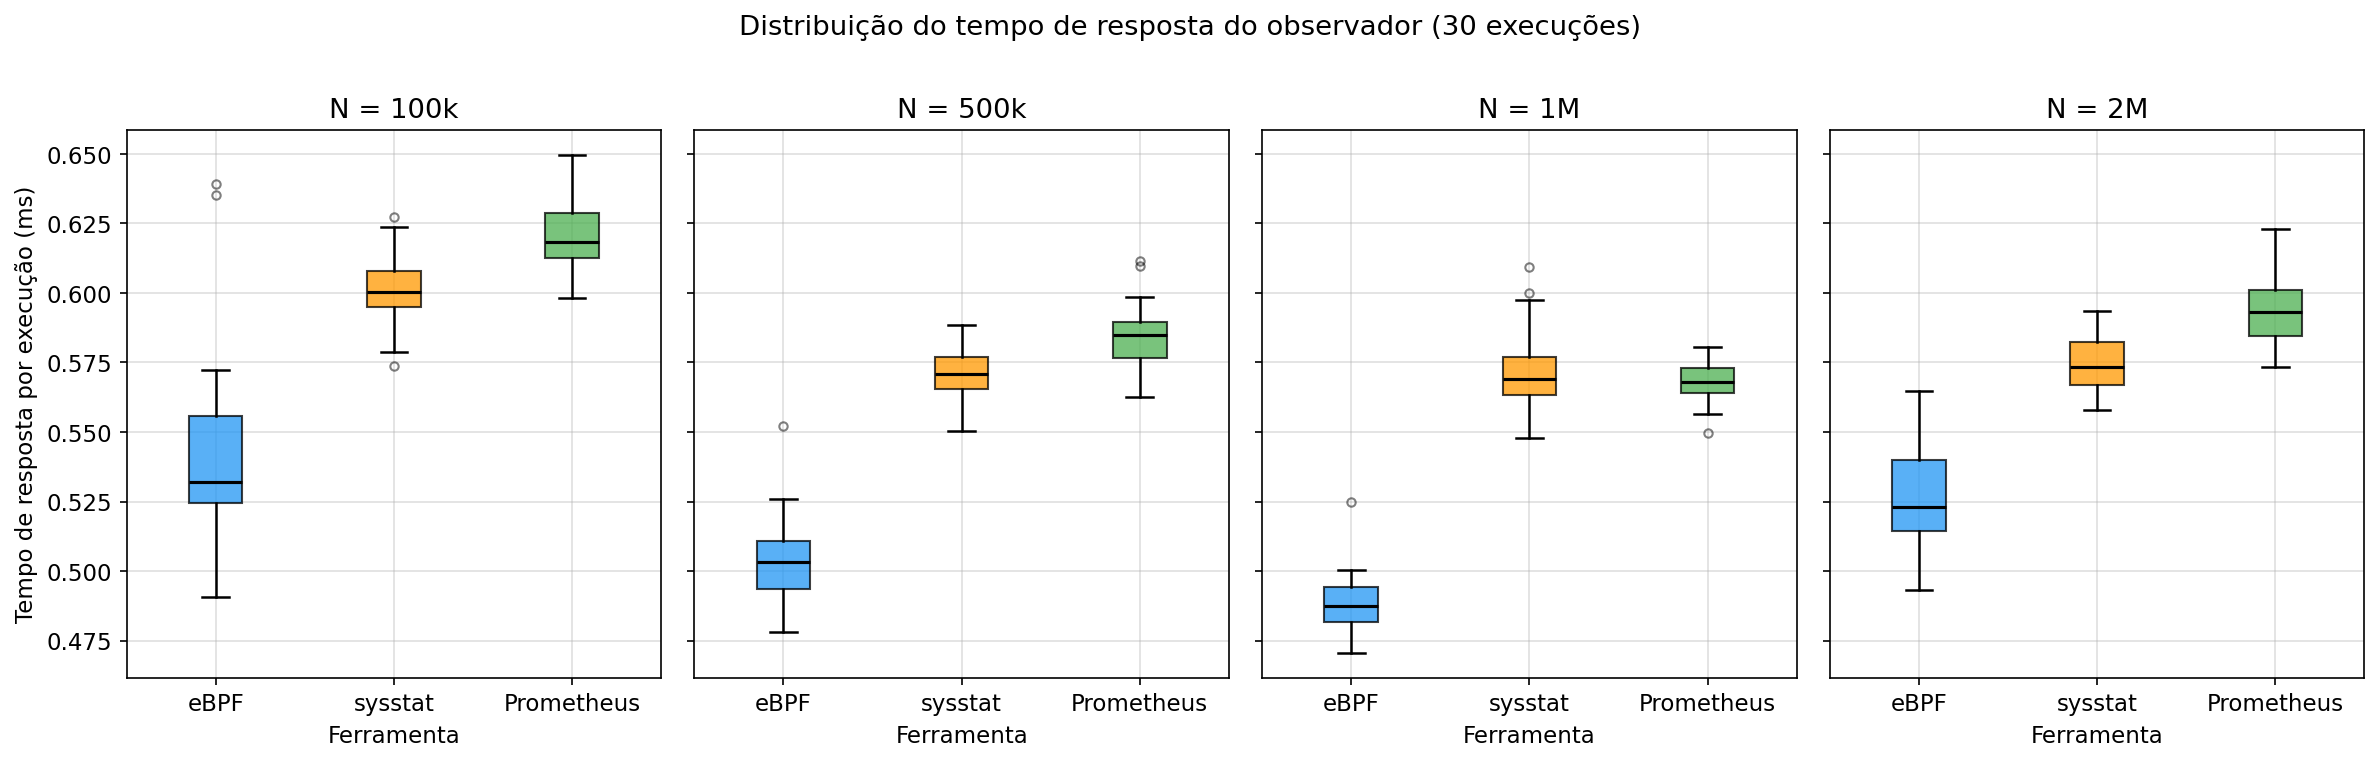
\includegraphics[width=\textwidth]{imagens/boxplot_tempo_resposta.png}
    \caption{Distribuição do tempo de resposta do observador por ferramenta e volume de mensagens.}
    \label{fig:rtt_boxplot}
\end{figure}

\FloatBarrier
\section{Consumo de CPU do WAF}

O consumo de CPU do processo WAF reflete o custo da inspeção de tráfego, idêntico nos três cenários por se tratar da mesma implementação. A Figura~\ref{fig:cpu_waf} mostra que, a partir de $N = 500$ mil, o WAF satura em torno de 107--109\% de uma \textit{thread} (valores superiores a 100\% indicam uso de mais de um núcleo lógico pelo \texttt{ThreadPoolExecutor}), sem diferença prática entre os coletores: os intervalos de confiança se sobrepõem em todos os volumes a partir desse ponto.

\begin{figure}[htbp]
    \centering
    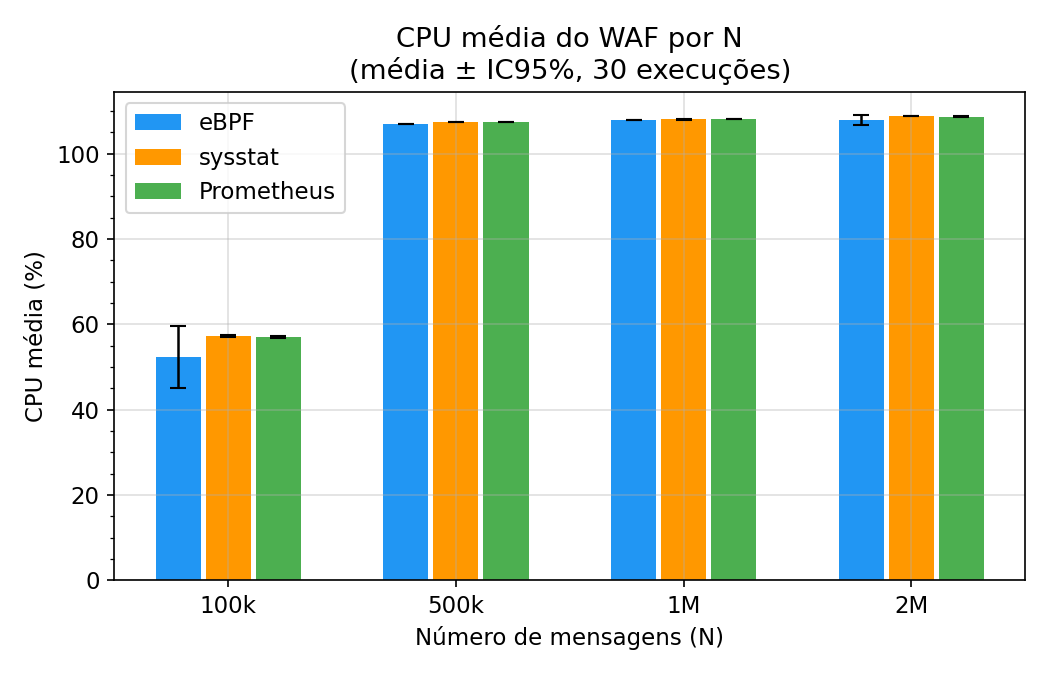
\includegraphics[width=0.85\textwidth]{imagens/cpu_waf.png}
    \caption{Consumo médio de CPU do processo WAF por volume de mensagens.}
    \label{fig:cpu_waf}
\end{figure}

A única exceção ocorre em $N = 100$ mil, em que o eBPF registrou um consumo médio de CPU inferior ($52{,}39\%$ contra $57{,}23\%$ do Sysstat e $57{,}04\%$ do Prometheus). Contudo, esse valor vem acompanhado de elevado intervalo de confiança ($\pm 7{,}28$, ante $\pm 0{,}20$ e $\pm 0{,}16$ das demais), refletindo a grande variabilidade do consumo de CPU em execuções curtas, em que o WAF não chega a operar em regime de saturação. Dada a sobreposição com a faixa de variação das outras ferramentas, não é possível atribuir essa diferença ao coletor. Em síntese, o consumo de CPU do WAF é dominado pela carga de inspeção e independe da abordagem de monitoramento adotada, resultado esperado, uma vez que nenhum dos coletores interfere no caminho de processamento das requisições.

\section{Consumo de Memória}

Esta seção analisa duas memórias distintas, com finalidades diferentes. A memória de interesse comparativo é a do \emph{próprio observador}: ela constitui o \textit{footprint} permanente da ferramenta de monitoramento --- a sobrecarga de memória que o coletor impõe apenas por estar em execução --- e é a dimensão em que as três abordagens mais se distinguem, o que justifica seu papel de variável dependente central (cf. Seção~\ref{subsec:requisitos_monitoramento}). A memória do WAF, por sua vez, é reportada como controle: por ser inerente à VNF e decorrer da mesma implementação em todos os cenários, serve para confirmar que a escolha do coletor não altera o consumo da função monitorada.

A Figura~\ref{fig:mem_observador} apresenta o consumo médio de memória RSS do processo observador, métrica em que se observa a separação mais nítida entre as três abordagens. O coletor Prometheus consome de $24{,}2$ a $24{,}8$ MB, aproximadamente 78\% acima do Sysstat ($13{,}5$ a $13{,}9$ MB) e 60\% acima do eBPF ($15{,}1$ a $15{,}2$ MB). Esse acréscimo decorre diretamente da biblioteca \texttt{prometheus\_client} e do servidor HTTP mantido em execução na porta 8000, ausentes nas demais abordagens.

\begin{figure}[htbp]
    \centering
    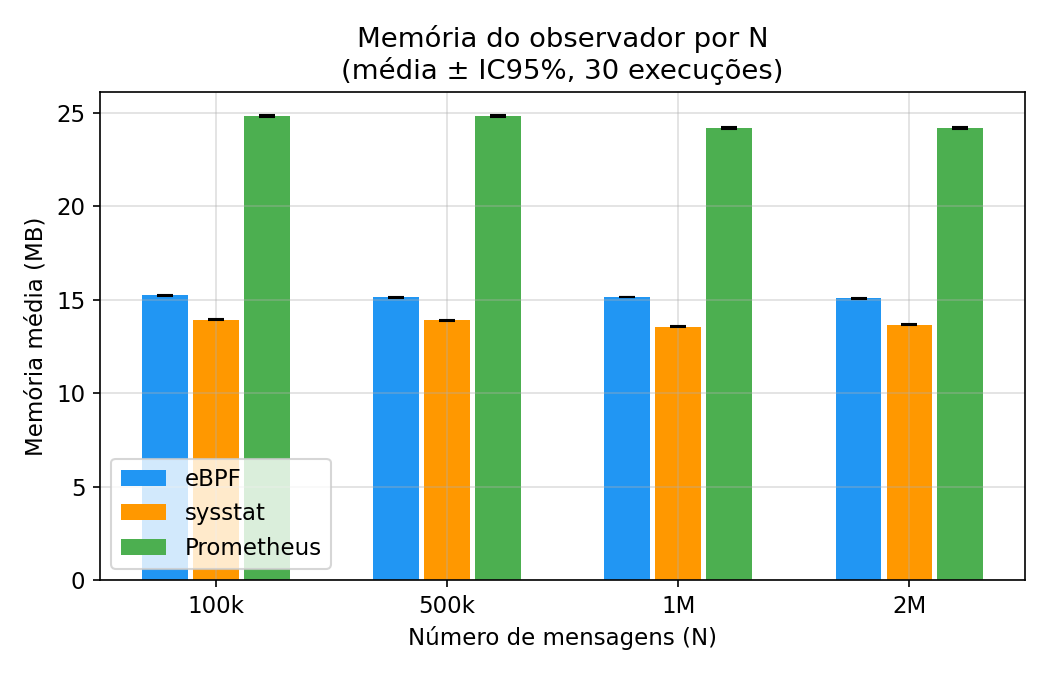
\includegraphics[width=0.85\textwidth]{imagens/memoria_observador.png}
    \caption{Consumo médio de memória RSS do processo observador por volume de mensagens (média $\pm$ IC95\%, 30 execuções).}
    \label{fig:mem_observador}
\end{figure}

Destaca-se que o consumo de memória de todos os coletores é praticamente constante ao longo dos quatro volumes de mensagens, com intervalos de confiança estreitos (inferiores a $0{,}2$ MB). Isso confirma que a memória do observador é determinada pela arquitetura de cada ferramenta, e não pelo volume de tráfego processado, comportamento esperado, dado que os coletores mantêm apenas contadores agregados e não armazenam o histórico de mensagens. O Sysstat apresentou o menor consumo, por depender unicamente de leituras de \texttt{/proc} e da biblioteca \texttt{psutil}; o eBPF situa-se ligeiramente acima, devido ao carregamento do programa BPF e dos mapas no \textit{kernel} pela \textit{libbpf}.

Quanto à memória do próprio WAF --- a VNF monitorada ---, os três cenários apresentaram valores semelhantes, crescendo de cerca de $28$ MB ($N = 100$ mil) para aproximadamente $50$ MB ($N = 2$ milhões), sem diferença atribuível ao coletor empregado. Esse crescimento acompanha o volume de tráfego processado e é inerente à VNF, não ao monitoramento, confirmando o papel de controle dessa medição.

\section{Consumo de CPU do Observador}

O consumo de CPU do próprio observador mostrou-se a métrica de medição mais delicada, devido à sua baixa magnitude frente ao ruído de amostragem. O resultado mais limpo foi obtido em $N = 100$ mil: o coletor eBPF consumiu, em média, apenas $0{,}05\% \pm 0{,}01$ de CPU, valor uma a duas ordens de grandeza inferior ao dos coletores em espaço de usuário ($4{,}66\%$ no Sysstat e $2{,}37\%$ no Prometheus) e, sobretudo, muito mais estável. Esse contraste é compatível com o argumento central de que a leitura de contadores diretamente dos mapas do \textit{kernel} é mais barata, em termos de CPU, do que a leitura periódica e o \textit{parsing} de arquivos do \texttt{/proc}; contudo, os intervalos de confiança do Sysstat ($\pm 6{,}54$) e do Prometheus ($\pm 4{,}72$) incluem o valor do eBPF, de modo que a diferença não é estatisticamente significativa.

Nos volumes maiores, entretanto, as medições de CPU do observador apresentaram desvios-padrão muito elevados em relação às médias (por exemplo, $0{,}82\% \pm 1{,}58$ no eBPF em $N = 1$ milhão), o que as torna pouco conclusivas isoladamente. Essa instabilidade decorre da granularidade da amostragem via \texttt{psutil} sobre intervalos curtos e da contenção de CPU entre os contêineres que compartilham os mesmos núcleos, conforme apontado nas limitações da metodologia. Por esse motivo, o consumo de CPU do observador é interpretado neste trabalho como evidência qualitativa complementar, e não como base para comparações quantitativas precisas entre as ferramentas.

\section{Métricas de Validação}

Além das métricas de comparação, registraram-se as métricas de validação descritas na metodologia, cujo objetivo é confirmar que as três ferramentas observaram a mesma carga de trabalho, e não discriminar as abordagens. O tempo médio de inspeção por carga convergiu para aproximadamente $0{,}081$ ms nas três abordagens (em $N = 1$ milhão, $0{,}0808$ ms no eBPF, $0{,}0815$ ms no Sysstat e $0{,}0807$ ms no Prometheus), confirmando que o custo unitário de processamento do WAF independe do coletor empregado --- comportamento esperado, dado que nenhuma abordagem interfere no caminho de inspeção das requisições.

Os contadores de bytes RX/TX, por outro lado, não são diretamente comparáveis entre as ferramentas, em razão da diferença no ponto de coleta. O coletor eBPF contabiliza exclusivamente o tráfego do WAF (porta de origem 8080), resultando em valores fortemente assimétricos --- em $N = 1$ milhão, cerca de $592$ MB recebidos contra apenas $8$ MB transmitidos, coerente com requisições volumosas e respostas curtas (\texttt{ALLOWED:OK} ou \texttt{BLOCKED}). Já o Sysstat e o Prometheus medem todo o tráfego da interface de \textit{loopback}, em que cada byte transmitido é também contabilizado como recebido, produzindo valores simétricos e mais elevados (RX $=$ TX, aproximadamente $618$ e $635$ MB, respectivamente). Essa diferença é inerente ao escopo de medição de cada abordagem, e não a um erro de contabilização; por isso, os bytes RX/TX são empregados apenas para caracterização, e não como critério de comparação entre as ferramentas.

\section{Síntese dos Resultados}

A Tabela~\ref{tab:sintese} resume o desempenho das três abordagens nas dimensões avaliadas. O eBPF foi a ferramenta de menor sobrecarga na métrica primária (tempo de resposta) em todos os volumes, com diferença estatisticamente significativa. Na CPU do próprio observador, as diferenças entre as ferramentas não foram conclusivas, devido à alta variabilidade entre as execuções. O Sysstat destacou-se pelo menor consumo de memória, enquanto o Prometheus apresentou o maior custo de memória, em razão do servidor HTTP, sem oferecer vantagem de desempenho no escopo testado, no qual o \textit{endpoint} de métricas permanece disponível, mas não é raspado ativamente.

\begin{table}[htbp]
\centering
\caption{Síntese comparativa das três abordagens de monitoramento.}
\label{tab:sintese}
\begin{tabularx}{\textwidth}{lXXX}
\hline
\textbf{Dimensão} & \textbf{eBPF} & \textbf{Sysstat} & \textbf{Prometheus} \\
\hline
Tempo de resposta (RTT UDP) & Menor & Intermediário & Maior \\
CPU do WAF & Equivalente & Equivalente & Equivalente \\
Memória do observador & Intermediária ($\sim$15 MB) & Menor ($\sim$14 MB) & Maior ($\sim$24 MB) \\
CPU do observador & Inconclusiva (mais estável em $N = 100$ mil) & Inconclusiva (ruidosa) & Inconclusiva (ruidosa) \\
\hline
\end{tabularx}
\end{table}

Os resultados confirmam a hipótese formulada na introdução: por operar em nível de \textit{kernel}, o eBPF apresenta menor tempo de resposta na coleta de métricas em comparação às abordagens de \textit{polling} em espaço de usuário, sem impor sobrecarga adicional ao WAF monitorado. A vantagem do eBPF no tempo de resposta, embora consistente e estatisticamente significativa, é de magnitude moderada (8\% a 15\%) e acompanhada de maior variabilidade entre execuções, fatores que devem ser ponderados na escolha da ferramenta em conjunto com os requisitos operacionais de cada cenário, discutidos no capítulo seguinte.

%\input{capítulos/3.ValidaçãoExperimental}
%\input{capítulos/4.ConsideraçõesFinais}

% ================================================================
% ELEMENTOS PÓS-TEXTUAIS
% ================================================================
\postextual

% --- Referências ---
\bibliography{referencias}

\end{document}
